\documentclass{article}
\usepackage[utf8]{inputenc}
\usepackage[margin=1in]{geometry}
\usepackage{todonotes}
\usepackage{tikz}
\usepackage{listings}
\usepackage{syntax}

% Insert liner notes using these commands
\newcommand{\nlsays}[1]{\todo[color=orange!40]{NL: #1}}
\newcommand{\sdsays}[1]{\todo[color=blue!40]{SD: #1}}
\newcommand{\wtsays}[1]{\todo[color=green!40]{WT: #1}}

\title{Matching Reference Behavior \\ by Simple Enumerative Synthesis}

\author{
  Souradeep Dutta \and
  Nicholas V. Lewchenko \and
  William Temple
}

\begin{document}

\maketitle

\nlsays{Just my first idea for the title; suggest your own}

\section{Introduction}
\label{sec:introduction}

\begin{figure}
  \centering
  \begin{tikzpicture}[node distance=5cm]
  \node (python) {{\Large \texttt{x ** y}}};
  \node (a) [above of=python,yshift=-4.2cm] {(a)};
  \node (theory) [right of=python] {{\LARGE $x^y$}};
  \node (b) [above of=theory,yshift=-4.2cm] {(b)};
  \node (x86) [right of=theory] {\lstinputlisting[basicstyle=\small]{exp.txt}};
  \node (c) [above of=x86,xshift=-2.3cm,yshift=-4cm] {(c)};
  \node [right of=python,xshift=-2.5cm] {{\LARGE$\rightarrow$}};
  \node [right of=theory,xshift=-3cm] {{\LARGE$\rightarrow$}};
\end{tikzpicture}

%%% Local Variables:
%%% mode: latex
%%% TeX-master: "paper"
%%% End:

  \caption{An exponentiation node in Python (a) translated into the
    arithmetic theory definition (b) and then x86 assembly
    implementation (c).}
  \label{fig:exp}
\end{figure}

Writing a compiler is difficult, in part because it requires a programmer to
implement the core functionality of their source language in one or more
assembly languages.

An assembly language is optimized for simple evaluation by a computer (simple
enough that \emph{hardware} can do it).

The consequence of this design requirement, illustrated in
Figure~\ref{fig:exp}, is that non-trivial assembly programs grow large, and
writing or reasoning about them is tedious and error-prone for a human.

The difference in complexity between the fully-specifying formal definition of
an operation and its assembly implementation is dramatic, suggesting that
computer assistance in this implementation process would significantly reduce
the necessary programming effort of a compiler programmer.

\section{Background}
\label{sec:background}

One of the promising ideas in Program synthesis is that of Sketching, explained
in \cite{phdthesis}. The idea in the Sketching program model is to allow the
programmer a robust scheme to tailor in the basic implementation outline while
leaving some of the details to the synthesizer. The programmer is expected to
come with the assertions in order to specify the correct behavior of the
program while giving the outline. The SKETCH Language is basically a layer on
top of a simple procedural language, with the only difference being the
introduction of the integer hole \textbf{??}.  Where the programmer expects the
integer hole to be replaced with a suitable integer.  \\ The "Hello World" in a
SKETCH programming model can be the following program, \\ \\ \textbf{void} main
(int x) \{ \\ int y = x * ?? ; \\ assert y == x + x; \\ \}

The three basic components of a SKETCH model are the following: i) the main
procedure , ii) holes, and iii) assertions.  The synthesizer is only allowed to
the fill up the holes with appropriate integer and not introduce any new lines. 

Another interesting idea in program synthesis is that of using enumerative
learning to come up with the expression. This idea is known by the name of
Syntax Guided Synthesis also known as \textbf{SyGuS} \cite{sygus}. Now, from a
top level the function synthesis problem is basically trying to find a function
$F$ such that some specification $\Phi$ is valid. The specification is expected
to capture the correctness of the desired program. For the syntax guided
synthesis problem it is constrained in the following ways:

\begin{itemize}
    \item The interpretation of the logical symbols and connectives
	are restricted to the background theory only.
    \item The logical formula $\Phi$ is only limited to be first order formulae in
	the back ground theoy.
    \item The possible functions are only restricted to be syntactic expressions
	generated by the grammar.
\end{itemize}

The main procedure in syntax guided synthesis is shown in Fig \ref{sygus_fig}.  
\begin{figure}
\label{sygus_fig}
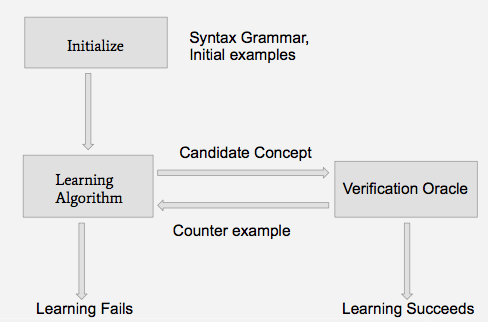
\includegraphics[scale = 0.8]{workflow.png}
\caption{SyGuS procedure \cite{sygus}}
\end{figure}

It essentially involves generating expressions and asking a verification oracle
to check the correctness of the generated expressions. If correct then , we
have the right function. Else, the oracle comes up with a counter example, and
the learning uses the Counter Example to refine it's search procedure. This
process is typically known in literature as a Counter Example Guided Inductive
Synthesis procedure or $CEGIS$.

This sort of enumerative synthesis algorithm though very simple to understand
and implement, can quickly become quite computationally expensive and
infeasible in practice when we try to generate even decent sized programs.

\section{Our Approach}
\label{sec:approach}

We have defined and implemented an enumerative synthesis procedure called
\textsc{SomeName} \nlsays{Will should give the tool a name.} for operation
implementations in a compiler for which a reference interpreter is available.
Our technique is source-language agnostic, using the preexisting reference
interpreter to produce a fixed set of test cases against which x86 programs
are sought.  This reference-guided partial verification reduces the complexity
of the technique.

\subsection{Virtual x86}

We define \textit{Virtual x86} (or vx86) to be a subset of the x86 language
where hardware registers have been replaced with infinitely many virtual,
indexed storage locations that behave exactly like hardware registers.  The
vx86 machine has the following properties:

\begin{itemize}
    \item Any instruction in vx86 has the same operating semantics as in
	regular x86.
    \item Only virtual registers are valid locations (there is no address
	space, nor any alternative addressing modes)
    \item No instructions which may alter the behavior of a future instruction
	are permitted
\end{itemize}

By limiting x86 in this way, we define a language which allows us to
recursively enumerate all possible programs and consider their behaviors
incrementally. Formally, a vx86 program has the following grammar:

\subsection{Generating Tests}

As our synthesis algorithm describes a general method for discovering programs
that satisfy a set of constraints, it is therefore also desirable to automate
test generation.  In our example scenario, we do this by interrogating a
reference interpreter using a random distribution of input values to produce
a suite of tests which are \textit{probably} comprehensive.

Given a $k$-ary operator, we will choose tests based on
\begin{itemize}
    \item all combinations of the numbers one and zero (based the fact that
	these are the multiplicative and additive identities, respectively),
	and
    \item a sample of sequences of $k$ values chosen by the result $f(x)=x^{9}$
	for random values of $x$, up to a certain threshold
\end{itemize}

Because the synthesis engine is slow, it is desirable to generate a suite of
test cases that covers both the boundary cases around zero and one as well as
a probabilistic subset of the larger space of integers in as few tests as
possible.

\begin{grammar}

<program> ::= <instruction> <program>
\alt <empty>

<instruction> ::= `mov' <register> <register>
\alt `add' <register> <register>
\alt `mul' <register> <register>
\alt `neg' <register>

<register> ::= `r' <natural-number>

\end{grammar}

\subsection{Synthesis}

Our synthesis algorithm is fully enumerative.  That is, it begins with an empty
program and considers every program that exists by enumerating all valid
derivations of new programs from existing programs.

We will say a program is a pair $(C,R)$, where $C$ is a sequence of
instructions following the grammar given above, and $R$ is a set of virtual
registers in use within $C$.  For synthesis of an arbitrary operator with $k$
operands (i.e. a $k$-ary operator), we will initialize our synthesis engine
with a set of candidate programs $P = {(\epsilon, \{r_{0}, r_{1}, r_{2} \ldots
r_{k-1}}\})$, containing only the null program with zero instructions and as
many virtual registers as our operator has inputs. We further initialize a set
$V = \{\}$, which is to store the set of program outputs we have seen, to be
empty.

\subsubsection{Validation}

During the validation step, we \textit{execute} each program $c \in P$ by
assigning the inputs of each test case to the first $k$ virtual registers and
simulating the result of executing each instruction in $c$, producing a
\textbf{signature}.  The signature of a program is the set of all register
assignments resulting from the execution of the program on each test.  If the
signature $S$ is in $V$, the set of visited program outputs, then we remove $c$
from $P$, as it is functionally equivalent to a program we have already
considered.  If $S$ is not in $V$, then $c$ will either be validated or
extended.

If the signature under consideration, $S$, contains any register which is
\textit{always} assigned to the result of its test case, then we say that $c$
satisfies the specification, and we accept $c$ as the correct solution and the
result of the synthesis problem.  If $c$ does not satisfy the specification,
then we add $S$ to $V$.

Once we have considered each program in $P$, and if no program was admitted as
the correct result, replace $P$ with $P'$ and continue to the next step,
program derivation.

\subsubsection{Derivation}

We begin derivation by constructing a set of next-generation programs $P' =
\{\}$ to be empty.  We then consider again, each program $c$ in $P$, and we
produce derivations of $c$ by considering modifications of $c$ according to the
following rules:

\begin{itemize}
    \item \textbf{Aliasing} one register to another, by adding a new virtual
	register $r_{j}$ to $c$, and inserting the instruction \texttt{mov
	$r_{i}$ $r_{j}$} to copies of $c$ for each virtual register $r_{i}$
	already in $c$.
    \item \textbf{Operating} over registers already in $c$, by considering all
	instructions other than \texttt{mov} and all combinations of registers
	in $c$ as operands. In other words, try every combination of registers
	with every possible instruction.
\end{itemize}

Every candidate derivation produced by the rules above will be added to $P'$.
Then, once we have considered all derivations of all programs and added them to
$P'$, we replace $P$ with $P'$ and return to the Validation step, repeating
this process until a correct program is found.

\section{Implementation & Evaluation}
\label{sec:evaluation}

\subsection{Implementation}
\label{sec:implementation}

We implemented a proof-of-concept of \textsc{SomeName} in Rust \ref{appendix-a}
\wtsays{what's the best way to inline this, or reference it}.  The
implementation follows the algorithm given above, but contains some
optimizations.  Most notably (from a performance standpoint), we compute the
results of each program incrementally (each Program contains a reference to its
parent program, its set of registers, and the instruction that makes it unique
from its parent), where each program is simulated only as an incremental change
from the results of the program that generated it.

\subsection{Example}

Consider the expression $x^{2} + y$.
\wtsays{Up to this point, I'm working on some examples.}

\section{Conclusion}
\label{sec:conclusion}

We believe that this technique presents a novel method for synthesizing
transformations from a high-level language to a machine language by leveraging
an existing interpreter (or any model by which expressions in the high-level
language may be automatically evaluated).  Our goal is not to eliminate the
work of writing a compiler, only to show that the most mundane aspects of
compiler design may be automated in some cases.  We are interested in how this
approach may be integrated with more conventional synthesis/verification
approaches involving, for example, SMT or SAT solvers, as our method is fast
for small operations though large programs remain intractable.  We believe that
this method may be useful for constructing the basic building blocks of a
compiled language, from which more advanced synthesis techniques may build more
comprehensive programs, utilizing the artifacts of our synthesis engine as
basic components.

\section*{Acknowledgements}

We thank Steven Malis (Software Engineer, Microsoft, Inc.) for his inspiration
and assistance with the incremental simulation optimization in our
proof-of-concept code, and for his permission to use this idea in our
implementation.

\bibliographystyle{plain}
\bibliography{references}	

\end{document}

